\subsection{Tree isomorphism in $\mathcal{O}(n)$}

\begin{frame}{Tree isomorphism}
    \begin{itemize}
        \item Trees are non-cyclic graphs
        \item Solution for the GI problem in linear time
        \item Good combination with modular decomposition
    \end{itemize}
\end{frame}

\begin{frame}{From graph to rooted tree}
    Algorithm by Bonany \cite{bonamy2010small}, returns the root that splits the tree in half
    \begin{enumerate}
        \item Choose an arbitrary root $r$
        \item Assign each vertex the weight of its induced subtree
        \item Start at $r$ and shift it with the neighbour that has weight \(>\frac{n}{2}\)
    \end{enumerate}
\end{frame}

\begin{frame}{Initial graph}
    \centering
    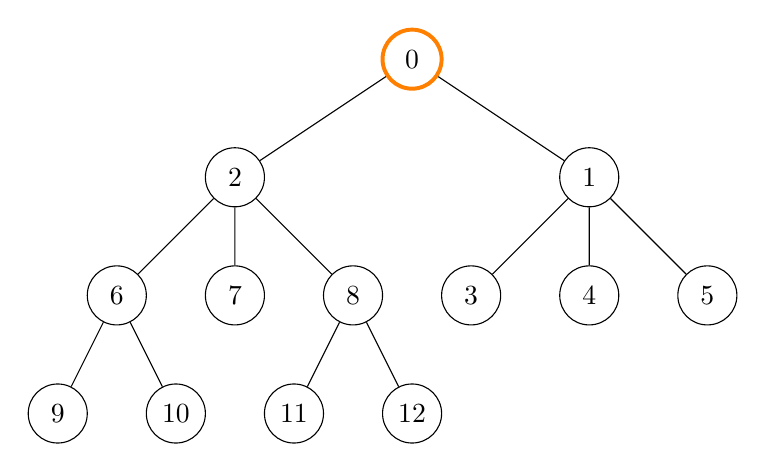
\begin{tikzpicture}[level/.style={sibling distance=15mm},  every node/.style={ minimum size=0.75cm}]
    \node [circle,draw=orange, line width = 0.5mm] (z){0}
        child {node [circle, draw] (y) {2}
            child {node [circle,draw] (a){6}
                child {node [circle,draw] (i) {9}}
                child {node [circle,draw] (j) {10}}
            }
            child {node [circle,draw] (b) {7}}
            child {node [circle,draw] (c) {8}
                child {node [circle,draw] (k) {11}}
                child {node [circle,draw] (l) {12}}
            }
        }
        child {node {} edge from parent[draw=none]}
        child {node {} edge from parent[draw=none]}
        child {node [circle,draw] (e) {1}
            child {node [circle,draw] (f) {3}}
            child {node [circle,draw] (g) {4}}
            child {node [circle,draw] (h) {5}}
        };
    \end{tikzpicture}    
\end{frame}

\begin{frame}{Rooted with assigned levels}
    \centering
    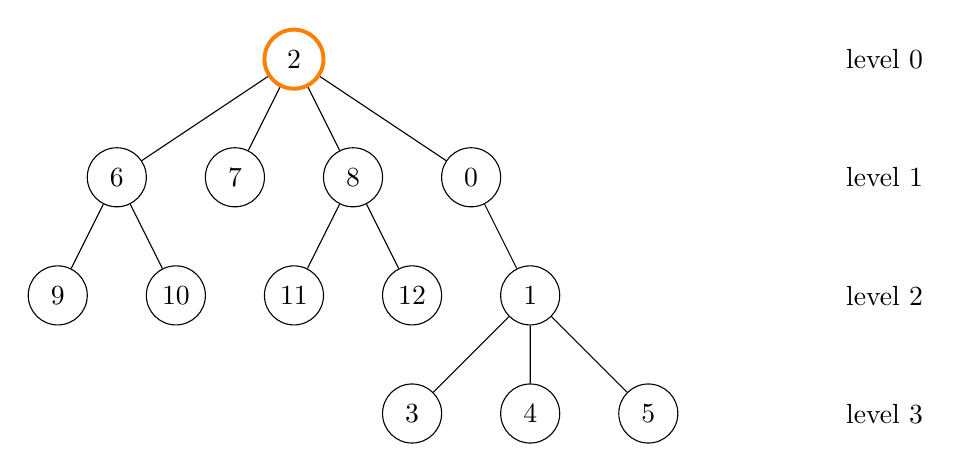
\begin{tikzpicture}[level/.style={sibling distance=15mm},  every node/.style={ minimum size=0.75cm}]
    \node [circle,draw=orange, line width = 0.5mm] (z){2}
        child {node [circle,draw] (a){6}
        child {node [circle,draw] (i) {9}}
        child {node [circle,draw] (j) {10}}
        }
        child {node [circle,draw] (b) {7}}
        child {node [circle,draw] (c) {8}
            child {node [circle,draw] (k) {11}}
            child {node [circle,draw] (l) {12}}
        }
        child {node [circle,draw] (d) {0}
            child {node (w) {} edge from parent[draw=none]}
            child {node [circle,draw] (e) {1}
                child {node [circle,draw] (f) {3}}
                child {node [circle,draw] (g) {4}}
                child {node [circle,draw] (h) {5}
                    child [grow=right] {node {} edge from parent[draw=none]
                        child [grow=right] {node (o) {level 3} edge from parent[draw=none]
                            child [grow=up] {node (p) {level 2} edge from parent[draw=none]
                                child [grow=up] {node (q) {level 1} edge from parent[draw=none]
                                    child [grow=up] {node {level 0} edge from parent[draw=none]}
                                }
                            }
                        }
                    }
                }
            }
        };
    \end{tikzpicture}
\end{frame}

\begin{frame}{Algorithm}
    \only<1>{In $\mathcal{O}(n)$, by Aho, Hopcroft and Ullman \cite{AhoHopcroftUllman}.}
    \only<2>{Assigned 0 to all leaves\\}
    \only<3>{Assign tuples to the vertices at level 2}
        \only<4>{Assign values to the distinct tuples, starting at 1, at level 2}
        \only<5>{Assign tuples to the vertices at level 1}
        \only<6>{Assign values to the distinct tuples}
        \only<7>{Assign tuples to the roots}
        \only<8>{Assign values to the root}
    \uncover<2>{\alert{Remark}: The orange indicates the final value of that node}
    \newcommand*\leafnodecolor{}
    \newcommand*\leaflinewidth{0.15mm}
    \newcommand*\leveltwonodecolor{}
    \newcommand*\leveltwolinewidth{0.15mm}
    \newcommand*\levelonenodecolor{}
    \newcommand*\levelonelinewidth{0.15mm}
    \newcommand*\rootnodecolor{}
    \newcommand*\rootlinewidth{0.15mm}
    \only<2->{\renewcommand*\leafnodecolor{orange}}
    \only<2->{\renewcommand*\leaflinewidth{0.5mm}}
    \only<4->{\renewcommand*\leveltwonodecolor{orange}}
    \only<4->{\renewcommand*\leveltwolinewidth{0.5mm}}
    \only<6->{\renewcommand*\levelonenodecolor{orange}}
    \only<6->{\renewcommand*\levelonelinewidth{0.5mm}}
    \only<8->{\renewcommand*\rootnodecolor{orange}}
    \only<8->{\renewcommand*\rootlinewidth{0.5mm}}
    \begin{center}
    \begin{tikzpicture}[level/.style={sibling distance=15mm},  every node/.style={ minimum size=0.75cm}]
    \node [circle,draw=\rootnodecolor, line width = \rootlinewidth] (z){\only<7>{(0,1,1,2)}\only<8>{1}}
        child {node [circle,draw=\levelonenodecolor, line width = \levelonelinewidth] (a){\only<5>{(0,0)}\only<6->{1}}
        child {node [circle,draw=\leafnodecolor, line width = \leaflinewidth] (i) {\only<2->0}}
        child {node [circle,draw=\leafnodecolor, line width = \leaflinewidth] (j) {\only<2->0}}
        }
        child {node [circle,draw=\leafnodecolor, line width = \leaflinewidth] (b) {\only<2->0}}
        child {node [circle, draw=\levelonenodecolor, line width = \levelonelinewidth] (c) {\only<5>{(0,0)}\only<6->{1}}
            child {node [circle,draw=\leafnodecolor, line width = \leaflinewidth] (k) {\only<2->0}}
            child {node [circle,draw=\leafnodecolor, line width = \leaflinewidth] (l) {\only<2->0}}
        }
        child {node [circle,draw=\levelonenodecolor, line width = \levelonelinewidth] (d) {\only<5>{(1)}\only<6->{2}}
            child {node (w) {} edge from parent[draw=none]}
            child {node [circle,draw=\leveltwonodecolor, line width = \leveltwolinewidth ] (e) {\only<3>{(0,0,0)}\only<4->{1}}
                child {node [circle,draw=\leafnodecolor, line width = \leaflinewidth] (f) {\only<2->0}}
                child {node [circle,draw=\leafnodecolor, line width = \leaflinewidth] (g) {\only<2->0}}
                child {node [circle,draw=\leafnodecolor, line width = \leaflinewidth] (h) {\only<2->0}
                    child [grow=right] {node {} edge from parent[draw=none]
                        child [grow=right] {node (o) {level 3} edge from parent[draw=none]
                            child [grow=up] {node (p) {level 2} edge from parent[draw=none]
                                child [grow=up] {node (q) {level 1} edge from parent[draw=none]
                                    child [grow=up] {node {level 0} edge from parent[draw=none]}
                                }
                            }
                        }
                    }
                }
            }
        };
    \end{tikzpicture}
    \end{center}
\end{frame}

\begin{frame}{Modular decomposition and trees}
\begin{itemize}
    \item Assign the same value to isomorphic modules, starting at the length of the vertices.
    \item Check if the modules in both graphs have the same tuples; otherwise their induced subtrees are different.
\end{itemize}
\end{frame}

